% Choose one to switch between slides and handout
%\documentclass[]{beamer}
\documentclass[handout]{beamer}

% Video Meta Data
\title{Bitcoin, Blockchain and Cryptoassets}
\subtitle{Elliptic Curves and ECDSA}
\author{Prof. Dr. Fabian Schär}
\institute{University of Basel}

% Config File
% Packages
\usepackage[utf8]{inputenc}
\usepackage{hyperref}
\usepackage{gitinfo2}
\usepackage{tikz}
\usepackage{amsmath}
\usepackage{bibentry}
\usepackage{xcolor}
\usepackage{colortbl} % Add colour to LaTeX tables
\usepackage{caption}
\usepackage[export]{adjustbox}
\usepackage{pgfplots} \pgfplotsset{compat = 1.17}

% Color Options
\definecolor{highlight}{rgb}{0.65,0.84,0.82}
\definecolor{focus}{rgb}{0.72, 0, 0}

% Beamer Template Options
\beamertemplatenavigationsymbolsempty
\setbeamertemplate{footline}[frame number]
\setbeamercolor{structure}{fg=black}
\setbeamercolor{footline}{fg=black}
\setbeamercolor{title}{fg=black}
\setbeamercolor{frametitle}{fg=black}
\setbeamercolor{item}{fg=black}
\setbeamercolor{}{fg=black}
\setbeamercolor{bibliography item}{fg=black}
\setbeamercolor*{bibliography entry title}{fg=black}
\setbeamertemplate{items}[square]
\setbeamertemplate{enumerate items}[default]
\captionsetup[figure]{labelfont={color=black},font={color=black}}
\captionsetup[table]{labelfont={color=black},font={color=black}}

\setbeamertemplate{bibliography item}{\insertbiblabel}

% Link Icon Command
\newcommand{\link}{%
    \tikz[x=1.2ex, y=1.2ex, baseline=-0.05ex]{%
        \begin{scope}[x=1ex, y=1ex]
            \clip (-0.1,-0.1)
                --++ (-0, 1.2)
                --++ (0.6, 0)
                --++ (0, -0.6)
                --++ (0.6, 0)
                --++ (0, -1);
            \path[draw,
                line width = 0.5,
                rounded corners=0.5]
                (0,0) rectangle (1,1);
        \end{scope}
        \path[draw, line width = 0.5] (0.5, 0.5)
            -- (1, 1);
        \path[draw, line width = 0.5] (0.6, 1)
            -- (1, 1) -- (1, 0.6);
        }
    }

% Read Git Data from Github Actions Workflow
% Defaults to gitinfo2 for local builds
\IfFileExists{gitInfo.txt}
	{\input{gitInfo.txt}}
	{
		\newcommand{\gitRelease}{(Local Release)}
		\newcommand{\gitSHA}{\gitHash}
		\newcommand{\gitDate}{\gitAuthorIsoDate}
	}

% Custom Titlepage
\defbeamertemplate*{title page}{customized}[1][]
{
  \vspace{-0cm}\hfill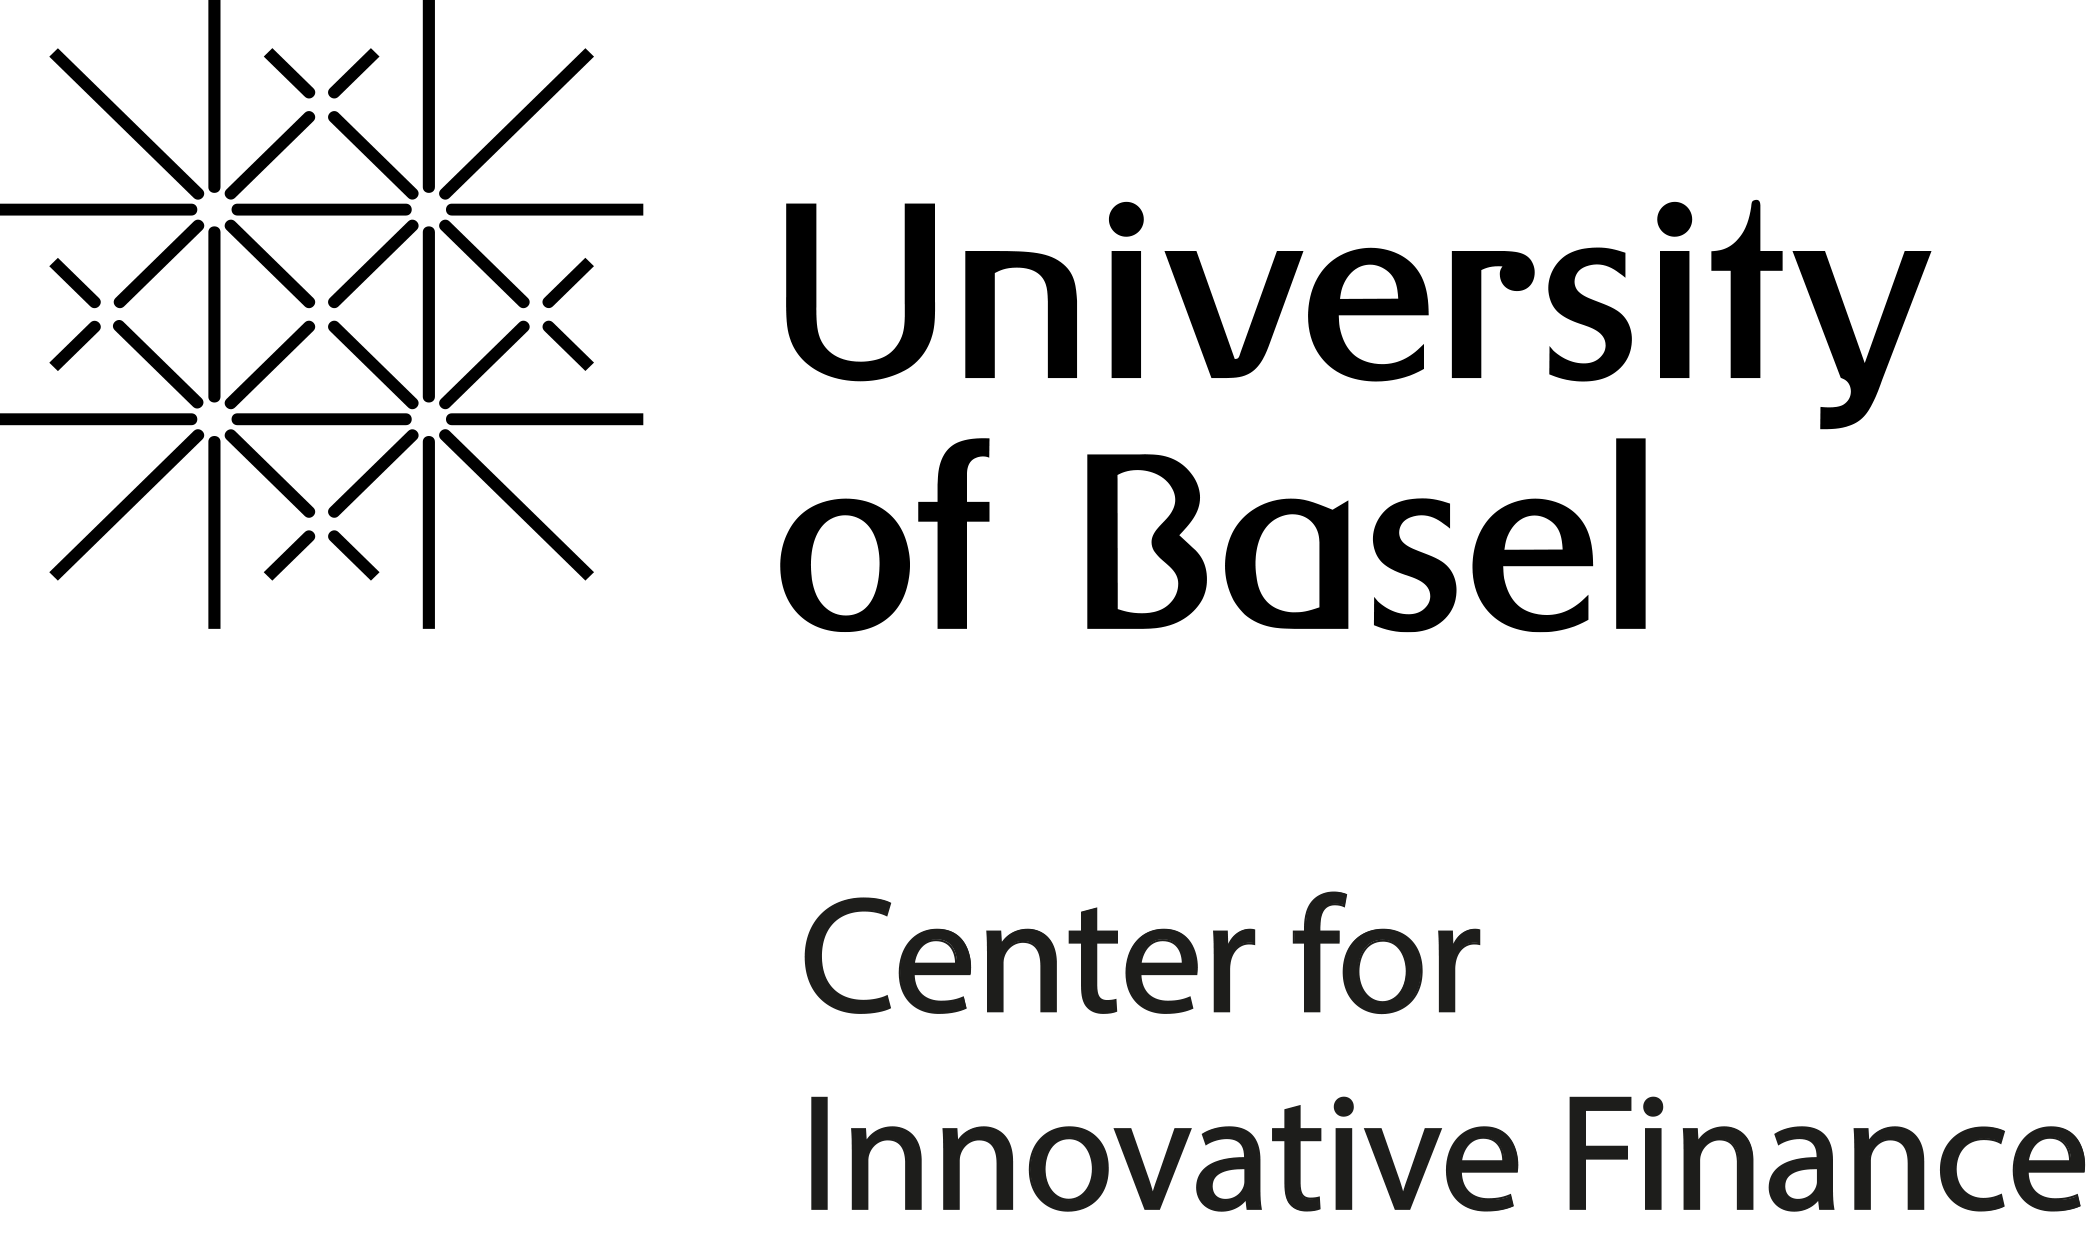
\includegraphics[width=2.5cm]{../config/logo_cif}
  
\includegraphics[width=1.9cm]{../config/seal_wwz}
  \\ \vspace{2em}
  \usebeamerfont{title}\textbf{\inserttitle}\par
  \usebeamerfont{title}\usebeamercolor[fg]{title}\insertsubtitle\par  \vspace{1.5em}
  \small\usebeamerfont{author}\insertauthor\par
  \usebeamerfont{author}\insertinstitute\par \vspace{2em}
  \usebeamercolor[fg]{titlegraphic}\inserttitlegraphic
    \tiny \noindent \texttt{Release Ver.: \gitRelease}\\ 
    \texttt{Version Hash: \gitSHA}\\
    \texttt{Version Date: \gitDate}\\ \vspace{1em}
  \link \href{https://github.com/cifunibas/Bitcoin-Blockchain-Cryptoassets/blob/main/slides/intro.pdf}
  {Get most recent version}\\
  \link \href{https://github.com/cifunibas/Bitcoin-Blockchain-Cryptoassets/blob/main/slides/intro.pdf}
  {Watch video lecture}\\ \vspace{1em}
  License: \texttt{Creative Commons Attribution-NonCommercial-ShareAlike 4.0 International}\\\vspace{2em}
  
\includegraphics[width = 1.2cm]{../config/license}
}

% tikzlibraries
\usetikzlibrary{decorations.pathreplacing}
\usetikzlibrary{decorations.markings}
\usetikzlibrary{positioning}

%caption font
\captionsetup{font=footnotesize}


%%%%%%%%%%%%%%%%%%%%%%%%%%%%%%%%%%%%%%%%%%%%%%
%%%%%%%%%%%%%%%%%%%%%%%%%%%%%%%%%%%%%%%%%%%%%%
\begin{document}

\thispagestyle{empty}
\begin{frame}[noframenumbering]
	\titlepage
\end{frame}

%%%
\begin{frame}{Example of an Elliptic Curve}
	\begin{columns}
		\begin{column}{0.5\textwidth}
			\begin{figure}
			\begin{tikzpicture}[scale = 0.7]
	\begin{axis}[xmin=-2.8,
            	xmax=2.8,
            	ymin=-2.8,
           		ymax=2.8,
            	xlabel={$x$},
            	ylabel={$y$},
            	scale only axis,
           		axis lines=middle,
         		domain=-1.76929235423863:3, % manually add min value to domain
            	samples=500,
            	smooth,
            	axis equal image=true,
        		]
		\addplot[focus]{sqrt(x^3 + -2*x + 2)};
		\addplot[focus]{-sqrt(x^3 + -2*x + 2)};		
	\end{axis}
\end{tikzpicture}	
				\caption*{Elliptic curve with $a = -2$, $b = 2$}
			\end{figure}	
		\end{column}
		\begin{column}{0.5\textwidth}
			Weierstrass equation:\\
			\vspace{1em}
			$y^2 = x^3 + ax + b$\\
			\vspace{2em}
			Non-singularity condition:\\
			\vspace{1em}
			$4a^3 + 27b^2 \neq 0$
		\end{column}
	\end{columns}
\end{frame}

\begin{frame}{Addition of Two Points}
	\begin{align*}
		P_1 &= (-1.5, \sqrt{1.625})\\
		P_2 &= (0, \sqrt{2})\\
		P_3 &= P_1 + P_2
	\end{align*}
	\begin{columns}
		\begin{column}{0.5\textwidth}
			\begin{figure}
				\begin{tikzpicture}[scale = 0.7]
	\begin{axis}[xmin=-2.8,
            	xmax=2.8,
            	ymin=-2.8,
           		ymax=2.8,
            	xlabel={$x$},
            	ylabel={$y$},
            	scale only axis,
           		axis lines=middle,
         		domain=-1.76929235423863:3, % manually add min value to domain
            	samples=500,
            	smooth,
            	axis equal image=true,
        		]
		\addplot[focus]{sqrt(x^3 + -2*x + 2)};
		\addplot[focus]{-sqrt(x^3 + -2*x + 2)};
		
		\only<2->{
			\draw [fill=black] (axis cs: -1.5, 1.2748) circle (2pt) node[left] {$P_1$};
			\draw [fill=black] (axis cs: 0, 1.4142) circle (2pt) node[above right] {$P_2$};
			\draw (axis cs: -1.5, 1.2748) -- (axis cs: 0, 1.4142);
		}
		
		\only<3->{
			\draw [fill=black] (axis cs: 1.5086, 1.5545) circle (2pt) node[right] {$-P_3$};
			\draw (axis cs: 0, 1.4142135) -- (axis cs: 1.5086, 1.5545);
		}
		
		\only<4->{
			\draw [dotted] (axis cs: 1.5086, 1.5545) -- (axis cs: 1.5086, -1.5545);
			\draw [fill=black] (axis cs: 1.5086, -1.5545) circle (2pt) node[right] {$P_3$};
		}
		
	\end{axis}
\end{tikzpicture}
			\end{figure}
		\end{column}
		\begin{column}{0.5\textwidth}
			\begin{align*}
				\uncover<5->{s &= \tfrac{y_{P_1} - y_{P_2}}{x_{P_1} - x_{P_2}} &= \hphantom{-} 0.0930\\[10pt]}
				\uncover<6->{x_{P_3} &= s^2 - (x_{P_1} + x_{P_2}) &= \hphantom{-} 1.5086\\[10pt]}
				\uncover<7->{y_{P_3} &= s(x_{P_1} - x_{P_3}) - y_{P_1} &= -1.5545}
			\end{align*}
		\end{column}
	\end{columns}
\end{frame}

\begin{frame}{Point Doubling}
	\begin{align*}
		P &= (-0.5, \sqrt{2.875})\\
		P + P &= 2P
	\end{align*}
	\begin{columns}
		\begin{column}{0.5\textwidth}
			\begin{figure}
				\begin{tikzpicture}[scale = 0.7]
	\begin{axis}[xmin=-2.8,
            	xmax=2.8,
            	ymin=-2.8,
           		ymax=2.8,
            	xlabel={$x$},
            	ylabel={$y$},
            	scale only axis,
           		axis lines=middle,
         		domain=-1.76929235423863:3, % manually add min value to domain
            	samples=500,
            	smooth,
            	axis equal image=true
        		]
        		
        % function: sqrt(x^3 + -2*x + 2)
       	\addplot[focus]{sqrt(x^3 + -2*x + 2)};
		\addplot[focus]{-sqrt(x^3 + -2*x + 2)};
		
        % x coordinate: -0.5 -> y coordinate: 1.6956
        % slope at x = -0.5: -0.368605
        % y intercept: 1.69558 + 0.5*(-0.368605) = 1.5113
        % line: 1.5112775 - 0.368605*x
        \only<2->{
        	\fill (axis cs: -0.5, 1.6956) circle (2pt) node[below left] {$P$};
			\addplot[black]{1.5113 - 0.3686*x};
		}

        % intersection:
        \only<3->{
        	\fill (axis cs: 1.1359, 1.0926) circle (2pt) node[right] {$-2P$};
        }
        
        \only<4->{
        	\fill (axis cs: 1.1359, -1.0926) circle (2pt) node[right] {$2P$};
        	\draw[dotted] (axis cs: 1.1359, 1.0926) -- (axis cs: 1.1359, -1.0926);
        }
        
	\end{axis}
\end{tikzpicture}
			\end{figure}
		\end{column}
		\begin{column}{0.5\textwidth}
			\begin{align*}
				\uncover<5->{s &= \tfrac{3x_P^2 + a}{2y_P} &= -0.3686\\[10pt]}
				\uncover<6->{x_{2P} &= s^2 - 2x_P &= \hphantom{-} 1.1359\\[10pt]}
				\uncover<7->{y_{2P} &= s(x_P - x_{2P}) - y_P &= -1.0926}
			\end{align*}
		\end{column}
	\end{columns}
\end{frame}

\begin{frame}{Elliptic Curves over Finite Fields}
	Bitcoin uses \texttt{secp256k1}:\ $y^2 = x^3 + 7\ (mod\ p)$ over ${\rm I\!F}_p$ where $p = 2^{256} - 2^{32} - 2^9 - 2^6 - 2^4 - 1$.\\
	\vspace{1em}
	\uncover<2->{\textbf{Simplified example:} $y^2 = x^3 + 7\ (mod\ 37)$ in ${\rm I\!F}_{37}$ \uncover<3->{with \textcolor{highlight}{$x = 5$}}}
	\begin{columns}[T]
		\begin{column}{0.5\textwidth}
			\uncover<2->{\begin{figure}
				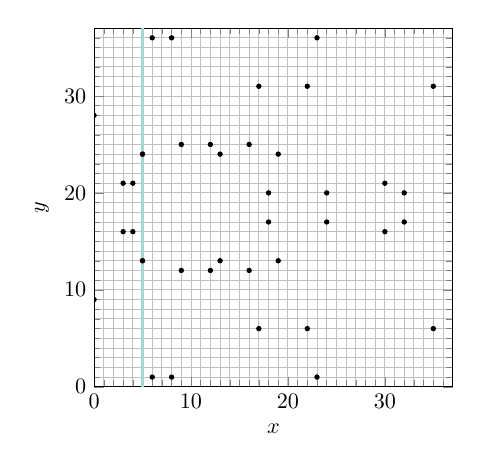
\begin{tikzpicture}[scale = 0.8]
	\begin{axis}[xmin=0, xmax=37,
				ymin=0, ymax=37,
            	xlabel={$x$},
            	ylabel={$y$},
         		domain=0:36,
            	axis equal image=true,
            	grid = both,
            	minor tick num=9
            	]
            	
        \only<3->{\draw [highlight, ultra thick] (axis cs: 5, 37) -- (axis cs: 5, 0);}
            	
        \draw [fill] (axis cs: 0, 9) circle (1pt){};
        \draw [fill] (axis cs: 0, 28) circle (1pt){};
        \draw [fill] (axis cs: 3, 16) circle (1pt){};
        \draw [fill] (axis cs: 3, 21) circle (1pt){};
        
        \draw [fill] (axis cs: 4, 16) circle (1pt){};
        \draw [fill] (axis cs: 4, 21) circle (1pt){};
        \alt<4->{\draw [fill = focus, draw = focus] (axis cs: 5, 13) circle (1pt){};}{\draw [fill, draw] (axis cs: 5, 13) circle (1pt){};}
        \alt<4->{\draw [fill = focus, draw = focus] (axis cs: 5, 24) circle (1pt){};}{\draw [fill, draw] (axis cs: 5, 24) circle (1pt){};}
        
        \draw [fill] (axis cs: 6, 1) circle (1pt){};
        \draw [fill] (axis cs: 6, 36) circle (1pt){};
        \draw [fill] (axis cs: 8, 1) circle (1pt){};
        \draw [fill] (axis cs: 8, 36) circle (1pt){};
        
        \draw [fill] (axis cs: 9, 12) circle (1pt){};
        \draw [fill] (axis cs: 9, 25) circle (1pt){};
        \draw [fill] (axis cs: 12, 12) circle (1pt){};
        \draw [fill] (axis cs: 12, 25) circle (1pt){};
        
        \draw [fill] (axis cs: 13, 13) circle (1pt){};
        \draw [fill] (axis cs: 13, 24) circle (1pt){};
        \draw [fill] (axis cs: 16, 12) circle (1pt){};
        \draw [fill] (axis cs: 16, 25) circle (1pt){};
        
        \draw [fill] (axis cs: 17, 6) circle (1pt){};
        \draw [fill] (axis cs: 17, 31) circle (1pt){};
        \draw [fill] (axis cs: 18, 17) circle (1pt){};
        \draw [fill] (axis cs: 18, 20) circle (1pt){};
        
        \draw [fill] (axis cs: 19, 13) circle (1pt){};
        \draw [fill] (axis cs: 19, 24) circle (1pt){};
        \draw [fill] (axis cs: 22, 6) circle (1pt){};
        \draw [fill] (axis cs: 22, 31) circle (1pt){};
        
        \draw [fill] (axis cs: 23, 1) circle (1pt){};
       \draw [fill] (axis cs: 23, 36) circle (1pt){};
       \draw [fill] (axis cs: 24, 17) circle (1pt){};
       \draw [fill] (axis cs: 24, 20) circle (1pt){};
       
       \draw [fill] (axis cs: 30, 16) circle (1pt){};
       \draw [fill] (axis cs: 30, 21) circle (1pt){};
       \draw [fill] (axis cs: 32, 17) circle (1pt){};
       \draw [fill] (axis cs: 32, 20) circle (1pt){};
       
       \draw [fill] (axis cs: 35, 6) circle (1pt){};
       \draw [fill] (axis cs: 35, 31) circle (1pt){};
  
	\end{axis}
\end{tikzpicture}
				\end{figure}
			}
		\end{column}
		\begin{column}{0.5\textwidth}
			\begin{align*}
					\uncover<4->{\textcolor{focus}{y}^2\ (mod\ 37) &\equiv \textcolor{highlight}{x}^3 + 7\ (mod\ 37)\\
					&\dots }\\
					\uncover<5->{\textcolor{highlight}{5}^3 + 7\ (mod\ 37) &= 132\ (mod\ 37)\\
					&= 21\\
					&\dots }\\
					\uncover<6->{\textcolor{focus}{y}^2\ (mod\ 37) &\equiv 21}\\
					\uncover<7->{\textcolor{focus}{13}^2\ (mod\ 37) &\equiv 21\\			
					\textcolor{focus}{24}^2\ (mod\ 37) &\equiv 21}
				\end{align*}
		\end{column}
	\end{columns}
\end{frame}

\begin{frame}{Modular Multiplicative Inverse}
	For our computations we often need the so-called modular multiplicative inverse.\\
	\vspace{1.5em}

	\uncover<2->{
		Regular division:\\
		$10 / 4 = 2.5$\\
		\vspace{1.5em}
	}
	
	\uncover<3->{
		Multiplicative inverse:\\
		$4/4 = 4 \cdot 4^{-1} = 1$\\
		$10 \cdot 4^{-1} = 2.5$\\
		\vspace{1.5em}
	}
	
	\uncover<4->{
		Modular multiplicative inverse:\\
		$\{4 \cdot x\}\ (mod\ 3) = 1$\\
		for $x = 1$\\
		because $4\ (mod\ 3) = 1$\\
	}
	
\end{frame}


\begin{frame}{ECDSA}
	\textbf{Simplified example:} Elliptic curve of order $N = 39$ with subgroups of the order $n = 13$:
	\begin{columns}[T]
		\begin{column}{0.5\textwidth}
			\uncover<2->{
				\begin{figure}
					\begin{tikzpicture}[scale = 0.8]
	\begin{axis}[xmin=0, xmax=37,
				ymin=0, ymax=37,
            	xlabel={$x$},
            	ylabel={$y$},
         		domain=0:36,
            	axis equal image=true,
            	grid = both,
            	minor tick num=9
            	]
           
        % show slope for 3G and all points from finite field
        \only<4-7>{
        	\draw [highlight, ultra thick] (axis cs: 7, 0) -- (axis cs: 36, 29);
        	
        	\draw [fill] (axis cs: 0, 9) circle (1pt){};
        	\draw [fill] (axis cs: 0, 28) circle (1pt){};
        	\draw [fill] (axis cs: 3, 16) circle (1pt){};
        	\draw [fill] (axis cs: 3, 21) circle (1pt){};
        
        	\draw [fill] (axis cs: 4, 16) circle (1pt){};
        	\draw [fill] (axis cs: 4, 21) circle (1pt){};
        	\draw [fill] (axis cs: 5, 13) circle (1pt){};
        	\draw [fill] (axis cs: 5, 24) circle (1pt){};
        	
        	\draw [fill] (axis cs: 6, 1) circle (1pt){};
       		\draw [fill] (axis cs: 6, 36) circle (1pt){};
        	\draw [fill] (axis cs: 8, 1) circle (1pt){};
        	\draw [fill] (axis cs: 8, 36) circle (1pt){};
        
        	\draw [fill] (axis cs: 9, 12) circle (1pt){};
        	\draw [fill] (axis cs: 9, 25) circle (1pt){};
        	\draw [fill] (axis cs: 12, 12) circle (1pt){};
        	\draw [fill] (axis cs: 12, 25) circle (1pt){};
        
        	\draw [fill] (axis cs: 13, 13) circle (1pt){};
        	\draw [fill] (axis cs: 13, 24) circle (1pt){};
        	\draw [fill] (axis cs: 16, 12) circle (1pt){};
        	\draw [fill] (axis cs: 16, 25) circle (1pt){};
        
        	\draw [fill] (axis cs: 17, 6) circle (1pt){};
        	\draw [fill] (axis cs: 17, 31) circle (1pt){};
        	\draw [fill] (axis cs: 18, 17) circle (1pt){};
        	\draw [fill] (axis cs: 18, 20) circle (1pt){};
        
        	\draw [fill] (axis cs: 19, 13) circle (1pt){};
        	\draw [fill] (axis cs: 19, 24) circle (1pt){};
        	\draw [fill] (axis cs: 22, 6) circle (1pt){};
        	\draw [fill] (axis cs: 22, 31) circle (1pt){};
        
       		\draw [fill] (axis cs: 23, 1) circle (1pt){};
       		\draw [fill] (axis cs: 23, 36) circle (1pt){};
       		\draw [fill] (axis cs: 24, 17) circle (1pt){};
       		\draw [fill] (axis cs: 24, 20) circle (1pt){};
       
       		\draw [fill] (axis cs: 30, 16) circle (1pt){};
       		\draw [fill] (axis cs: 30, 21) circle (1pt){};
       		\draw [fill] (axis cs: 32, 17) circle (1pt){};
       		\draw [fill] (axis cs: 32, 20) circle (1pt){};
       
       		\draw [fill] (axis cs: 35, 6) circle (1pt){};
       		\draw [fill] (axis cs: 35, 31) circle (1pt){};
        }
        
        % show second part of slope for 3G
        \only<5-7>{
        	\draw [highlight, ultra thick] (axis cs: 0, 30) -- (axis cs: 6, 36);
        }
        
        % show point -3G and dotted line to 3G
        \only<6-7>{
        	\draw [dotted, highlight, ultra thick] (axis cs: 6, 36) -- (axis cs: 6, 1);
        	\draw [fill = focus, draw = focus] (axis cs: 6, 36) circle (1pt) node[below left, focus]{\scriptsize{$-3G$}};
        }
        
        \draw [fill = focus, draw = focus] (axis cs: 8, 1) circle (1pt) node[above right, focus]{\scriptsize{$G$}};
        
        \only<3->{
        	\draw [fill = focus, draw = focus] (axis cs: 24, 17) circle (1pt) node[right, focus]{\scriptsize{$2G$}};
        	\draw [black, ->, shorten <= 0.1cm, shorten >= 0.1cm] (axis cs: 8, 1) to[out=0,in=-110] (axis cs: 24, 17);
        }
        
        \only<7->{
        	\draw [fill = focus, draw = focus] (axis cs: 6, 1) circle (1pt) node[left, focus]{\scriptsize{$3G$}};
        	\draw [black, ->, shorten <= 0.1cm, shorten >= 0.1cm] (axis cs: 24, 17) to[out=-150,in=45] (axis cs: 6, 1);
        }
        
        \only<8->{
        	\draw [fill = focus, draw = focus] (axis cs: 23, 36) circle (1pt) node[below, focus]{\scriptsize{$4G$}};
        	\draw [black, ->, shorten <= 0.1cm, shorten >= 0.1cm] (axis cs: 6, 1) to[out=135,in=180] (axis cs: 23, 36);
        }
        
        \only<9->{
        	\draw [fill = focus, draw = focus] (axis cs: 32, 17) circle (1pt) node[below, focus]{\scriptsize{$5G$}};
        	\draw [black, ->, shorten <= 0.1cm, shorten >= 0.1cm] (axis cs: 23, 36) to[out=0,in=0] (axis cs: 32, 17);
        }
        
        \only<10->{
        	\draw [fill = focus, draw = focus] (axis cs: 18, 17) circle (1pt) node[below left, focus]{\scriptsize{$6G$}};
        	\draw [black, ->, shorten <= 0.1cm, shorten >= 0.1cm] (axis cs: 32, 17) to[out=155,in=15] (axis cs: 18, 17);
        }
        
        \only<11->{
        	\draw [fill = focus, draw = focus] (axis cs: 18, 20) circle (1pt) node[above left, focus]{\scriptsize{$7G$}};
        	\draw [black, ->, shorten <= 0.1cm, shorten >= 0.1cm] (axis cs: 18, 17) -- (axis cs: 18, 20);
        }
        
        \only<12->{
        	\draw [fill = focus, draw = focus] (axis cs: 32, 20) circle (1pt) node[above, focus]{\scriptsize{$8G$}};
        	\draw [black, ->, shorten <= 0.1cm, shorten >= 0.1cm] (axis cs: 18, 20) to[out=-15,in=-165] (axis cs: 32, 20);
        }
        
        \only<13->{
        	\draw [fill = focus, draw = focus] (axis cs: 23, 1) circle (1pt) node[above, focus]{\scriptsize{$9G$}};
        	\draw [black, ->, shorten <= 0.1cm, shorten >= 0.1cm] (axis cs: 32, 20) to[out=0,in=0] (axis cs: 23, 1);
        }

		\only<14->{
			\draw [fill = focus, draw = focus] (axis cs: 6, 36) circle (1pt) node[left, focus]{\scriptsize{$10G$}};
        	\draw [black, ->, shorten <= 0.1cm, shorten >= 0.1cm] (axis cs: 23, 1) to[out=180,in=-135] (axis cs: 6, 36);
        }

		\only<15->{
			\draw [fill = focus, draw = focus] (axis cs: 24, 20) circle (1pt) node[right, focus]{\scriptsize{$11G$}};
        	\draw [black, ->, shorten <= 0.1cm, shorten >= 0.1cm] (axis cs: 6, 36) to[out=-45,in=150] (axis cs: 24, 20);
        }

		\only<16->{
			\draw [fill = focus, draw = focus] (axis cs: 8, 36) circle (1pt) node[below right, focus]{\scriptsize{$12G$}};
        	\draw [black, ->, shorten <= 0.1cm, shorten >= 0.1cm] (axis cs: 24, 20) to[out=110,in=0] (axis cs: 8, 36);
		}
        
	\end{axis}
\end{tikzpicture}
				\end{figure}
			}
		\end{column}
		\begin{column}{0.5\textwidth}
			\vspace{1em}
			\uncover<2->{\textbf{e.g.\ \textcolor{focus}{$G = (8, 1)$}:}\\
			\uncover<3->{The cyclic subgroup consists of \textcolor{focus}{$\{0, G, 2G, ..., (n-1)G\}$}}}
			\uncover<3->{
				\alt<4-7>{
					\begin{align*}
						s &= \{(1 - 17) \cdot (8 - 24)^{-1}\}\ (mod\ 37)\\
						&= \{(-16) \cdot (30)\}\ (mod\ 37) \\
						&= 1\\
						\textcolor{focus}{x_{3G}} &= \{1 - (8 + 24)\}\ (mod\ 37)\\
						&= 6\\
						\textcolor{focus}{y_{3G}} &= \{1 \cdot (8 - 6) - 1\}\ (mod\ 37)\\
					 	&= 1
					\end{align*}
				}{
					\begin{align*}
						s &= \{3 \cdot 8^2 \cdot (2)^{-1}\}\ (mod\ 37)\\
						&= \{3 \cdot 8^2 \cdot 19\}\ (mod\ 37)\\
						&= 22\\
						\textcolor{focus}{x_{2G}} &= \{22^2 - 2 \cdot 8\}\ (mod\ 37)\\
						&= 24\\
						\textcolor{focus}{y_{2G}} &= \{22 \cdot (8 - 24) - 1\}\ (mod\ 37)\\
					 	&= 17
					\end{align*}
				}
			}
		\end{column}
	\end{columns}
\end{frame}

\begin{frame}{Key Generation}
	\textbf{Simplified example: \textcolor{focus}{$k_{prv} = 9$} and \textcolor{focus}{$G = (8,1)$}}
	\begin{columns}
		\begin{column}{0.5\textwidth}
			\uncover<2->{
				\begin{figure}
					\begin{tikzpicture}[scale = 0.8]
	\begin{axis}[xmin=0, xmax=36,
				ymin=0, ymax=36,
            	xlabel={$x$},
            	ylabel={$y$},
         		domain=0:36,
            	axis equal image=true,
            	grid = both,
            	minor tick num=9
            	]
            	            	
        \draw [fill = focus, draw = focus] (axis cs: 8, 1) circle (1pt) node[above right, focus]{\scriptsize{$G$}};
        
        \only<3->{
        	\draw [fill = focus, draw = focus] (axis cs: 24, 17) circle (1pt) node[right, focus]{\scriptsize{$2G$}};
        	\draw [black, ->, shorten <= 0.1cm, shorten >= 0.1cm] (axis cs: 8, 1) to[out=0,in=-110] (axis cs: 24, 17);
        }
        
        \only<4->{       
        	\draw [fill = focus, draw = focus] (axis cs: 23, 36) circle (1pt) node[below, focus]{\scriptsize{$4G$}};
        	\draw [black, ->, shorten <= 0.1cm, shorten >= 0.1cm] (axis cs: 24, 17) to[out=135,in=180] (axis cs: 23, 36);
        }
                             
        \only<5->{
        \draw [fill = focus, draw = focus] (axis cs: 32, 20) circle (1pt) node[above, focus]{\scriptsize{$8G$}};
        \draw [black, ->, shorten <= 0.1cm, shorten >= 0.1cm] (axis cs: 23, 36) to[out=0,in=180] (axis cs: 32, 20);
       	}
       	
       	\only<6->{
        	\draw [fill = focus, draw = focus] (axis cs: 23, 1) circle (1pt) node[above, focus]{\scriptsize{$9G$}};
        	\draw [black, ->, shorten <= 0.1cm, shorten >= 0.1cm] (axis cs: 32, 20) to[out=0,in=0] (axis cs: 23, 1);
        }
        
	\end{axis}
\end{tikzpicture}
				\end{figure}
			}
		\end{column}
		\begin{column}{0.5\textwidth}
			\uncover<2->{\textbf{From $k_{prv}$ to $K_{pub}$ using the double and add algorithm:}
				\begin{enumerate}
					\item<3-> Double: $2 \circ G = 2G$
					\item<4-> Double: $2 \circ 2G = 4G$
					\item<5-> Double: $2 \circ 4G = 8G$
					\item<6-> Add: $8G + G = 9G$
				\end{enumerate}
				\uncover<7->{$\rightarrow$ Four steps only! Algorithm runtime: $\mathcal{O}(\log_{2}n)$}
			}
		\end{column}
	\end{columns}
\end{frame}

\begin{frame}{Elliptic Curve Discrete Logarithm Problem}
	\begin{figure}
		\begin{tikzpicture}
	\begin{axis}[xmin = 0, xmax = 20,
						ymin = 0, ymax = 20,
						width = 0.9\textwidth,
						height = 0.7\textheight,
						legend pos = north west,
						xtick distance = 10,
						ytick distance = 10,
						grid = both,
						xlabel = {$n$},
						ylabel = {Algorithm runtime}
						]
						
			\addplot[focus, domain = 0:20, very thick] {ln(x)/ln(2)};
			\addplot[highlight, domain = 0:20, very thick] {x};
		
			\legend{
				$\mathcal{O}(\log_{2}n)$, 
				$\mathcal{O}(n)$
			};
			
	\end{axis}
\end{tikzpicture}	
	\end{figure}
\end{frame}

\begin{frame}{Example: Signature}
	\textbf{Simplified example:}\\
	\begin{columns}[T]
		\begin{column}{0.3\textwidth}
			\begin{itemize}
				\item $y^2 = x^3 + 7$
				\item $G = (8, 1)$
				\item $k_{prv} = 9$
				\item $K_{pub} = (23, 1)$
				\item $t = 4$
			\end{itemize}
		\end{column}
		\begin{column}{0.7\textwidth}
			\begin{enumerate}
				\item<2-> Choose random number, e.g.\ $i = 7$
				\item<3-> Compute
				\begin{enumerate}[a.]
					\item<3-> $P = i \cdot G = 7G = (18,20)$\\
						\vspace{0.5em}
					\item<4-> $r = x_P\ (mod\ n) = 18\ (mod\ 13) = 5$\\
						\vspace{0.5em}
					\item<5-> $s = \{i^{-1} (t + r \cdot k_{prv})\}\ (mod\ n)$\\
						$\hphantom{s } = \{2 \cdot (4 + 5 \cdot 9)\}\ (mod\ 13)$\\
						$\hphantom{s } = 7$
				\end{enumerate}
				\item<6-> Send
				\begin{enumerate}[a.]
					\item<6-> $(r, s) = (5, 7)$\\
					\vspace{0.5em}
					\item<7-> $t = 4$\\
					\vspace{0.5em}
					\item<8-> $K_{pub} = (23, 1)$\\
					\vspace{0.5em}
				\end{enumerate}
			\end{enumerate}
		\end{column}
	\end{columns}
\end{frame}

\begin{frame}{Example: Verification}
	\textbf{Simplified example:}\\
	\begin{columns}[T]
		\begin{column}{0.3\textwidth}
				\begin{itemize}
					\item $y^2 = x^3 + 7$
					\item $G = (8, 1)$
					\item $K_{pub} = (23, 1)$
					\item $t = 4$
					\item $(r, s) = (5, 7)$
				\end{itemize}
		\end{column}
		\begin{column}{0.7\textwidth}
			\begin{enumerate}
				\item<2-> Compute\\
				\begin{enumerate}[a.]
					\item<2-> $\{u_1 = (s^{-1}t)\}\ (mod\ n) = 8\ mod\ 13 = 8$\\
					\vspace{0.5em}
					\item<3-> $\{u_2 = (s^{-1}r)\}\ (mod\ n) = 10\ mod\ 13 = 10$\\
					\vspace{0.5em}
					\item<4-> $P = u_1 \circ G + u_2 \circ K_{pub}$\\
					 $\hphantom{P }  = 8G + 10 \circ (23, 1)$\\
					 $\hphantom{P } = (32, 20) + (8, 36)$\\
					 $\hphantom{P } = (18, 20)$
				\end{enumerate}
				\item<5-> Check authenticity: $x_P\ mod\ n = r$\\
				Here: $18\ (mod\ 13) = 5$
			\end{enumerate}
		\end{column}
	\end{columns}
	\vspace{1.5em}
	\uncover<6->{$\rightarrow$ The private key is never revealed.}\\
	\uncover<7->{$\rightarrow$ \href{https://github.com/cifunibas/Bitcoin-Blockchain-Cryptoassets/blob/main/assets/scripts/ecdsa_example.py}{\link Python script to signature and verification examples}}
\end{frame}


%%%
%\begin{frame}%[allowframebreaks]
%\frametitle{References and Recommended Reading}
%	\bibliographystyle{amsplain}
%	\bibliography{../assets/bib/refs}
%\end{frame}


\end{document}